\begin{table}[t]
\caption{
Kendall's rank coefficient between GoP \& intelligibility severity levels. A higher absolute value indicates a stronger correlation between the two variables.
}
\vspace{1em}
\label{tab:results}
\centering
\resizebox{0.48\textwidth}{!}
{

\begin{tabular}{c|c|c|c|c|c}
\hline
Method & Norm. & Scoring Func. & English & Korean & Tamil \\
\hline
\multirow{3}{*}{Baseline} 
& None & GMM \cite{witt2000phone,hmm-gop} & -0.2049 & -0.5237 & -0.3571 \\
& None & NN \cite{hu2015improved} & -0.1536 & -0.4687 & -0.4003 \\
& Prior & DNN-GoP \cite{hu2015improved} & -0.1836 & -0.4237 & -0.4681 \\
\hline
\multirow{12}{*}{Proposed} 
& \multirow{4}{*}{None}  & Entropy & -0.1831 & -0.2643 & -0.3251  \\
&  & Margin & -0.1628 & -0.4434 & -0.4445 \\
&  & MaxLogit & -0.2164 & -0.5440 & -0.5786 \\
&  & LogitMargin & -0.1732 & -0.4753 & -0.5158 \\
\cline{2-6}
& \multirow{4}{*}{Scale} & Entropy & -0.1755 & -0.1974 & -0.2263 \\
&  & Margin & -0.1260 & -0.4444 & -0.4210\\
&  & MaxLogit & -0.2164 & -0.5440 & -0.5786 \\
&  & LogitMargin & -0.1732 & -0.4753 & -0.5158\\
\cline{2-6}
& \multirow{4}{*}{Prior} & Entropy & -0.1833 & -0.2645 & -0.3254  \\
&  & Margin & -0.1630 & -0.4432 & -0.4447\\
&  & \textbf{MaxLogit} & \textbf{-0.2165} & \textbf{-0.5442} & \textbf{-0.5788}\\
&  & LogitMargin & -0.1733 & -0.4753 & -0.5160\\
\hline
\end{tabular}
}
\vspace{-1em}
\end{table}

% GMM-GOP \cite{hmm-gop} & & &\\
%
\section{Experimental results} \label{sec:results}
\subsection{Correlation between GoPs and intelligilbity scores}
\Cref{tab:results} demonstrates the performances of both baseline and proposed experiments, with the best performance indicated in bold.
GoP with prior normalized MaxLogit performed the best on all the languages among the baselines and the UQ methods, achieving $-21.65\%$, $-54.42\%$, $-57.88\%$ correlation, for English, Korean, and Tamil, respectively.
% We assume the lowest correlation was attained for the English dataset due to the alignment errors.

The results of the baseline experiments show that GMM-GoP has the highest correlation for English and Korean at $-20.49\%$ and $-52.37\%$, respectively, while DNN-GoP performs best for Tamil with a correlation of $-46.81\%$.
For the proposed experiments, GoP without normalization generally shows lower performance than the baseline, except for MaxLogit-based GoP. 
Additionally, while scaling normalization has minimal impact, prior normalization has a positive effect on GoP performance for all languages. 
Furthermore, when entropy-based, probability-based (Margin), and logit-based (MaxLogit, LogitMargin) GoP variants are compared, the logit-based GoPs show the highest correlations to the intelligibility scores.
% To sum up, according to the experimental results, prior-normalized logit-based GoP yields the best performance for dysarthric speech intelligibility assessment.
Additionally, performances on English are notably lower than that of Tamil and Korean.
We suspect that automatically generated alignment causes the degradation to occur \cite{mathad2021impact}, for the severe cases where alignment becomes much more challenging.
We aim to mitigate this issue in our future work.

% \input{figures/phone_diagram}

\subsection{Analysis on phonemes}
\Cref{figs:phones} illustrates the GoP distribution between two Korean phonemes \textipa{/i/} and \textipa{/m/}.
While the distribution of \textipa{/i/} differs significantly, the distribution of \textipa{/m/} is similar across all severity levels.
This finding suggests that certain phonemes have more impact power for severity levels based on speech intelligibility, which is consistent with previous findings \cite{quintas2022automatic}.

\begin{figure}[t] %%% t: top, b: bottom, h: here
\centering
\subfloat[Korean phoneme \textipa{/i/}.]{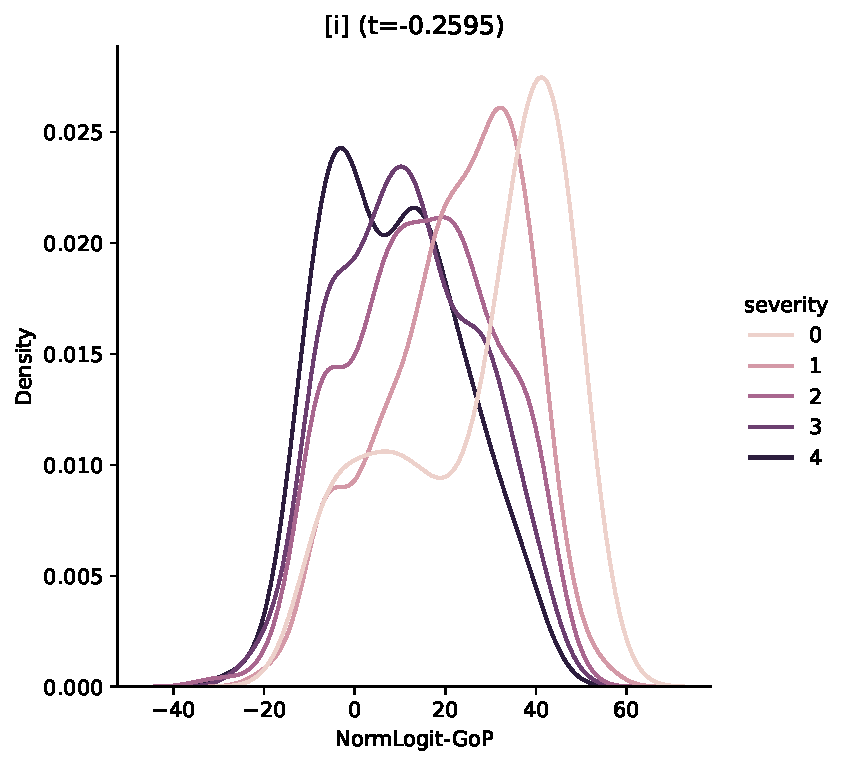
\includegraphics[width=0.43\columnwidth]{figures/korean_i.pdf}}
\subfloat[Korean phoneme \textipa{/m/}.]{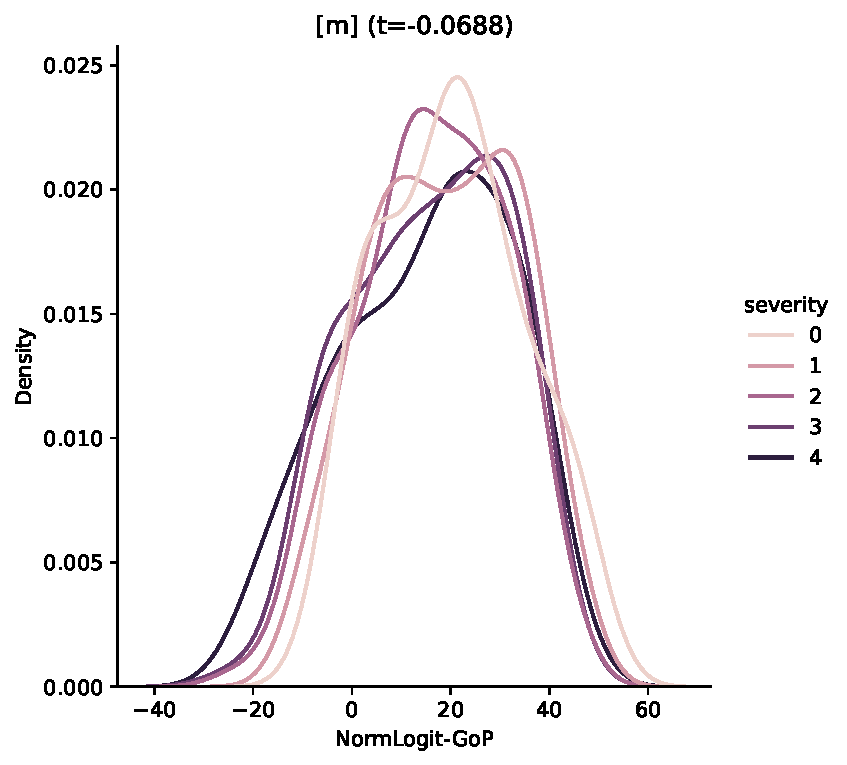
\includegraphics[width=0.43\columnwidth]{figures/korean_m.pdf}}
\vspace{1em}
\caption{
Kendall's $\tau$ distributions for two phonemes by severity.
0:healthy, 1:mild, 2:mild-to-mod., 3:mod.-to-sev., 4:severe.
}
\vspace{-1em}
\label{figs:phones}
\end{figure}

% As certain phonemes have a more significant impact on speech intelligibility than others, 
Identifying which phoneme pronunciation scores highly correlate to speech intelligibility can be useful in the clinical scenario, such as diagnosis and treatment.
For example, as demonstrated in \Cref{figs:samplewise_phones}, one can pinpoint the mispronounced phonemes within a single utterance.


Further, we conduct a quantitative analysis on which phoneme scores highly correlate to speech intelligibility by languages.
Kendall's $\tau$ is calculated for each phoneme between our best-performing Prior+MaxLogit GoP score and the intelligibility scores.
The top-5 phonemes based on correlation are as follows- English: \textipa{/a\textsci/},\textipa{/\textesh/},\textipa{/a\textupsilon/},\textipa{/z/},\textipa{/\textdyoghlig/}; Korean:\textipa{/i/},\textipa{/s/},\textipa{/n/},\textipa{/a/},\textipa{/\textturnv/}; Tamil:\textipa{/\textrtails/},\textipa{/h/},\textipa{/\textteshlig/},\textipa{/z/},\textipa{/a\textsci/}.
In summary, fricative sounds (\textipa{/s/},\textipa{/\textrtails/},\textipa{/\textesh/},\textipa{/z/}) strongly correlates to speech intelligibility across languages, consistent with the previous results \cite{hernandez2019acoustic}.
Affricates (\textipa{/\textteshlig/},\textipa{/\textdyoghlig/}) and diphthongs (\textipa{/a\textsci/},\textipa{/a\textupsilon/}) were shared as the top-5 phoneme list for English and Tamil.
This can be explained by the complexity in the articulation of affricates and diphthongs leading to difficulties in correct pronunciation for speakers with lower speech intelligibility.
On the other hand, Korean showed higher correlations for nasal (\textipa{/n/}) and monophthongs (\textipa{/a/},\textipa{/i/},\textipa{/\textturnv/}).
This may be again related to the movement of the articulators, such as the tongue, velum, and jaw.
We additionally provide the correlation scores of all the phonemes in our repository.\footref{footnote:repo_url}
